% !TeX root = ../../main.tex
\chapter{仿真实验}[Numerical Experiments]\label{cw:sec:simulation}
本节先汇报 Gordon 基准冻结数据集上的滤波对照、参数消融与串行计时结果，再通过零过程噪声 Logistic 模型考察粒子贫化与误差分解；运行环境见表~\ref{cw:tab:sim-environment}。

\begin{table}[htbp]
\centering
\caption{运行环境}
\label{cw:tab:sim-environment}
\wuhao
\begin{tabular}{ll}
\toprule[1.5pt]
项目 & 配置 \\
\midrule[1pt]
CPU & AMD Ryzen 9 9955HX3D，16 核 32 线程 \\
系统可见内存 & 60.50 GiB \\
操作系统 & Ubuntu 24.04.4 LTS \\
数值内核 & C++17 / Eigen 3.4.0 \\
数值精度 & 双精度 \\
\bottomrule[1.5pt]
\end{tabular}
\end{table}

\section{模型与实验简介}
采用 Gordon 等的一维非线性基准\cite{gordon1993novel}，并按本实验设置选取初始分布：
\begin{equation}\label{cw:eq:sim-model}
\begin{aligned}
&X_k=\tfrac12X_{k-1}+\frac{25X_{k-1}}{1+X_{k-1}^2}+8\cos\!\bigl(1.2(k-1)\bigr)+N_{x,k},\\
&Y_k=X_k^2/20+N_{y,k},\quad
X_0\sim\mathcal N(0,2),\ N_{x,k}\sim\mathcal N(0,10),\ N_{y,k}\sim\mathcal N(0,1).
\end{aligned}
\end{equation}
高斯记号 $\mathcal N(\mu,\sigma^2)$ 的第二参数表示方差。状态每步演化，仅在 $k\in m\mathbb N$ 时提供观测，$m$ 表示观测间隔。

本次仿真实验中，不同算法与间隔复用同一批冻结真值和全量观测。
实验中的 BPF 采用系统重采样\cite{doucet2001sequential}, ETPF 采用熵正则化输运；数值实现使用稳定化 Sinkhorn\cite{schmitzer2019stabilized} 与边际修正\cite{altschuler2017nearlinear}, 表中的结果对应这些实现。
对照方法包括扩展 Kalman 滤波（EKF）\cite{bar2001estimation}、自举粒子滤波（BPF）\cite{gordon1993novel}、集合 Kalman 滤波（EnKF）\cite{evensen2003ensemble}及熵正则化集合变换粒子滤波（ETPF）\cite{reich2013nonparametric,cuturi2013sinkhorn}。


本实验取 $B=8$ 条轨迹，每条含 $K=100$ 个状态步。记第 $b$ 条轨迹的真值为 $x_k^{(b)}$，在线估计为 $\widehat x_k^{+,(b)}$；缺测步取预测均值。定义
\begin{equation}\label{cw:eq:sim-metrics}
\begin{aligned}
&\mathrm{RMSE}_k=\sqrt{\frac1B\sum_{b=1}^{B}(\widehat x_k^{+,(b)}-x_k^{(b)})^2},\quad
\mathrm{RMSE}=\sqrt{\frac1K\sum_{k=1}^{K}\mathrm{RMSE}_k^2},\\
&S_X=\sqrt{\frac1{BK}\sum_{b,k}(x_k^{(b)})^2},\qquad
\mathrm{NRMSE}=100\,\mathrm{RMSE}/S_X\ (\%).
\end{aligned}
\end{equation}

\begin{table}[htbp]
\centering
\caption{精度与串行计算开销，$m=1,N=500$，ETPF 取 $\varepsilon=1$。时间为每条轨迹三次重复的中位数，再对 $8$ 条轨迹取均值 $\pm$ 样本标准差}
\label{cw:tab:sim-runtime}
\wuhao\setlength{\tabcolsep}{5pt}
% !TeX root = ../../../main.tex
\begin{tabular}{lrrr}
\toprule[1.5pt]
算法 & 每步内核时间 $\downarrow$ ($\mu$s) & 相对误差 $\downarrow$ (\%) & 未收敛率 $\downarrow$ \\
\midrule[1pt]
EKF & $\mathbf{0.104}\pm 0.003$ & $167.87$ & -- \\
BPF & $38.013\pm 0.100$ & $\mathbf{43.83}$ & -- \\
EnKF & $49.680\pm 0.125$ & $48.32$ & -- \\
ETPF & $28293.091\pm 2576.275$ & $44.43$ & 23.13\% \\
\bottomrule[1.5pt]
\end{tabular}

\end{table}

EKF 最快但误差最大；BPF 在该设置下兼具较低误差与计算成本。ETPF 每步约 $28.29$ ms，远高于 BPF 的 $38.01\,\mu$s。

表~\ref{cw:tab:sim-runtime} 的未收敛率指 Sinkhorn 在 $1000$ 次迭代内未达到边缘容差 $10^{-8}$ 的观测更新次数占比，收敛率为其补数。


% 先输出此前表格，并为小节标题预留空间；本组图表按阅读顺序落位。
\FloatBarrier
\Needspace{10\baselineskip}
\section{时序误差分析}
\suppressfloats[t]

表~\ref{cw:tab:sim-accuracy} 与图~\ref{cw:fig:sim-time} 显示，本组数据中 BPF 与 ETPF 精度接近，EnKF 略差。

\begin{table}[htbp]
\centering
\caption{全时域 RMSE $\downarrow$，括号内为 NRMSE $\downarrow$。上下标为整条轨迹 bootstrap（$1000$ 次）所得 95\% 区间相对中心值的偏移；按未舍入值标粗每列最优。}
\label{cw:tab:sim-accuracy}
\wuhao\setlength{\tabcolsep}{7pt}
% !TeX root = ../../../main.tex
\begin{tabular}{lcccc}
\toprule[1.5pt]
算法 & $m=1$ & $m=2$ & $m=4$ & $m=8$ \\
\midrule[1pt]
EKF & \begin{tabular}[c]{@{}c@{}}$17.80_{-1.74}^{+1.38}$\\$(167.87\%)$\end{tabular} & \begin{tabular}[c]{@{}c@{}}$22.80_{-3.26}^{+2.61}$\\$(215.01\%)$\end{tabular} & \begin{tabular}[c]{@{}c@{}}$40.85_{-24.81}^{+25.07}$\\$(385.27\%)$\end{tabular} & \begin{tabular}[c]{@{}c@{}}$16.67_{-3.19}^{+3.07}$\\$(157.17\%)$\end{tabular} \\[2pt]
BPF & \begin{tabular}[c]{@{}c@{}}$\mathbf{4.65}_{-0.58}^{+0.59}$\\$(\mathbf{43.83}\%)$\end{tabular} & \begin{tabular}[c]{@{}c@{}}$6.44_{-0.57}^{+0.59}$\\$(60.76\%)$\end{tabular} & \begin{tabular}[c]{@{}c@{}}$\mathbf{7.46}_{-0.34}^{+0.22}$\\$(\mathbf{70.34}\%)$\end{tabular} & \begin{tabular}[c]{@{}c@{}}$8.14_{-0.45}^{+0.37}$\\$(76.78\%)$\end{tabular} \\[2pt]
EnKF & \begin{tabular}[c]{@{}c@{}}$5.12_{-0.62}^{+0.61}$\\$(48.32\%)$\end{tabular} & \begin{tabular}[c]{@{}c@{}}$6.71_{-0.58}^{+0.65}$\\$(63.26\%)$\end{tabular} & \begin{tabular}[c]{@{}c@{}}$7.94_{-0.29}^{+0.31}$\\$(74.85\%)$\end{tabular} & \begin{tabular}[c]{@{}c@{}}$8.39_{-0.26}^{+0.23}$\\$(79.16\%)$\end{tabular} \\[2pt]
ETPF & \begin{tabular}[c]{@{}c@{}}$4.71_{-0.66}^{+0.66}$\\$(44.43\%)$\end{tabular} & \begin{tabular}[c]{@{}c@{}}$\mathbf{6.41}_{-0.56}^{+0.56}$\\$(\mathbf{60.43}\%)$\end{tabular} & \begin{tabular}[c]{@{}c@{}}$7.50_{-0.36}^{+0.22}$\\$(70.76\%)$\end{tabular} & \begin{tabular}[c]{@{}c@{}}$\mathbf{8.14}_{-0.45}^{+0.35}$\\$(\mathbf{76.76}\%)$\end{tabular} \\[2pt]
\bottomrule[1.5pt]
\end{tabular}

\end{table}

\begin{figure}[!htb]
\centering
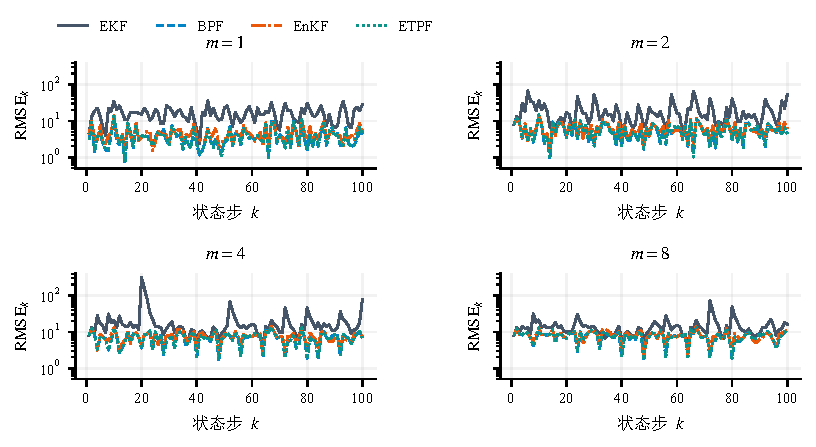
\includegraphics[width=0.84\linewidth]{figs/completed_work/rmse_time.pdf}
\caption{逐时刻跨轨迹 RMSE，$N=500,\varepsilon=1$。各子图采用相同对数纵轴。}
\label{cw:fig:sim-time}
\end{figure}

\begin{figure}[!htb]
\centering
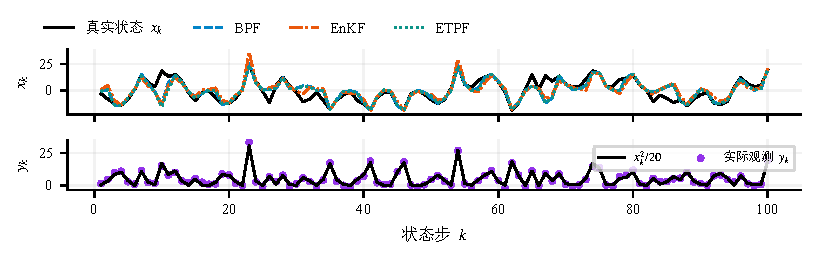
\includegraphics[width=0.84\linewidth]{figs/completed_work/trajectory.pdf}
\caption{首条轨迹的状态与观测，$m=1$；下图对照 $y_k$ 与 $x_k^2/20$。}
\label{cw:fig:sim-observation}
\end{figure}

\FloatBarrier
\section{粒子数，正则强度与计算开销}

\begin{figure}[!htb]
\centering
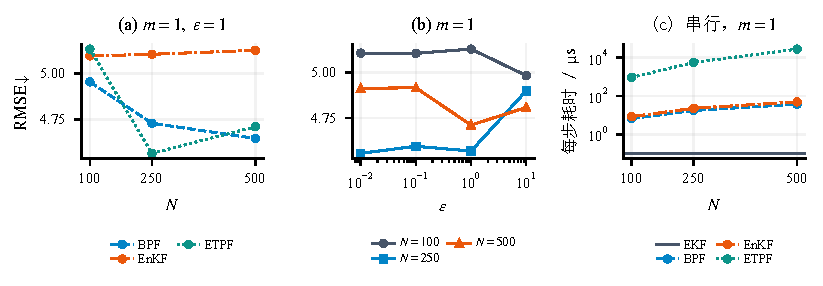
\includegraphics[width=0.88\linewidth]{figs/completed_work/ablation_runtime.pdf}
\caption{单因素切片均取 $m=1$。(a) 固定 $\varepsilon=1$ 比较 $N$；(b) 比较 ETPF 的 $\varepsilon$；(c) 相同冻结数据上的串行单核每步内核耗时，对 ETPF 固定 $\varepsilon=1$。}
\label{cw:fig:sim-ablation}
\end{figure}

在所测试的三个粒子数量下，BPF 的 RMSE 随 $N$ 增大而下降；固定 $\varepsilon=1$ 时，ETPF 的 RMSE 未呈严格单调下降。该现象限于本组有限轨迹与参数设置，尚不能据此判断两者相对 Bayes 最优估计的渐近差距。在本次消融范围内，正则化强度 $\varepsilon$ 对相对误差的影响较小，其选择仍需结合计算开销和收敛情况。

\begin{figure}[!htb]
\centering
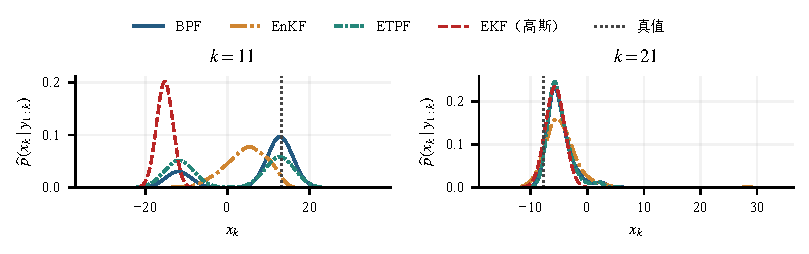
\includegraphics[width=0.88\linewidth]{figs/completed_work/posterior_density.pdf}
\caption{首条轨迹的后验密度估计，$m=1,N=500,\varepsilon=1$。}
\label{cw:fig:sim-density}
\end{figure}

图~\ref{cw:fig:sim-density} 中，$k=11$ 时 BPF 与 ETPF 均呈双峰，而 EKF 的高斯近似仅保留单峰。
$k=21$ 时各估计的主峰位置接近，但峰宽仍有差异。
在上述 Gordon 基准及当前参数设置下，ETPF 继承了 PF 的非高斯表示能力，但更高的计算开销未带来明显精度优势。

% 先收束 Gordon 基准图表，避免混入后续 Logistic 实验。
\FloatBarrier
% !TeX root = ../../../main.tex
\section{零过程噪声 Logistic 模型：粒子贫化与稳健性}\label{cw:sec:sim-logistic}
考虑确定性混沌状态演化与非线性观测：
\begin{equation}\label{cw:eq:sim-logistic-model}
\begin{aligned}
&X_k=4X_{k-1}(1-X_{k-1}),\quad X_k\in[0,1],\\
&Y_k=h(X_k)+N_{y,k},\quad h(x)=x^2,\quad
X_0\sim U[0,1],\quad N_{y,k}\sim\mathcal N(0,0.1).
\end{aligned}
\end{equation}
每步均有观测，取 $N=128$，共 $64$ 条独立观测路径，每条 $1000$ 步，每条路径独立运行算法 $32$ 次。观测噪声方差为 $0.1$；BPF 采用每步多项重采样，ETPF 采用一维无正则最优输运。不同粒子位置数按双精度数值精确去重统计。

图~\ref{cw:fig:sim-logistic-robustness} 比较两种算法的误差与粒子多样性，四项误差统计见表~\ref{cw:tab:sim-logistic-errors}。

\begin{table}[!htb]
\centering\wuhao
\caption{Logistic 模型的四项误差与实测总 MSE，第 $1$--$1000$ 步平均。}
\label{cw:tab:sim-logistic-errors}
% !TeX root = ../../../main.tex
\begin{tabular}{lrr}
\toprule[1.5pt]
误差项 & BPF & ETPF \\
\midrule[1pt]
不可约 Bayes 误差 & 0.048755 & 0.048755 \\
算法偏差平方 & 0.075192 & 0.002376 \\
算法随机波动 & 0.123494 & 0.021038 \\
当前重采样扰动 & $4.48\times10^{-6}$ & $5.03\times10^{-31}$ \\
\midrule[1pt]
实测总 MSE & 0.247544 & 0.072128 \\
\bottomrule[1.5pt]
\end{tabular}

\end{table}
表\ref{cw:tab:sim-logistic-errors}评估了重采样后均值 $\hat X_k=X_k^+\mathbf1_N/N$，四项对应式~\eqref{cw:eq:four-errors}。理论分解是总体期望恒等式；表中各项为有限路径与重复运行的估计，Bayes 风险由数值参考后验近似，因此，四项之和与实测总 MSE 未必逐位相等。

\begin{figure}[!htb]
\centering
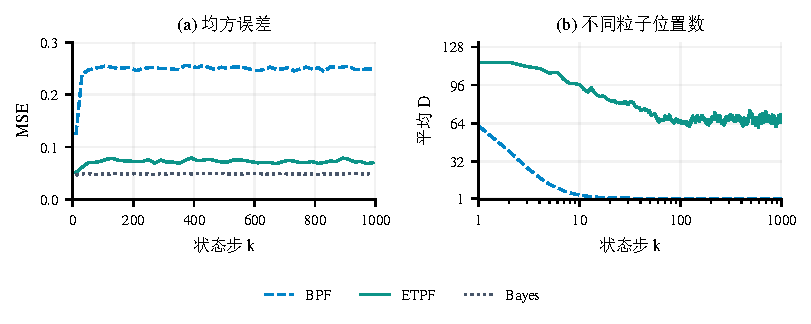
\includegraphics[width=0.88\linewidth]{figs/completed_work/logistic_robustness.pdf}
\caption{同一批运行的误差与粒子多样性。(a) 每 $20$ 步分段平均的 MSE 与 Bayes 参考风险；(b) 重采样后不同位置数的跨运行平均，横轴取对数以显示早期贫化。}
\label{cw:fig:sim-logistic-robustness}
\end{figure}
% 学位论文版式中正常续排结论，避免旧的预留空间指令将短段落推到新页。
BPF 的 $2048$ 次运行均贫化为单点；ETPF 在这批运行中没有单点贫化，末步平均保留 $69.67$ 个不同位置，总 MSE 较 BPF 降低 $70.9\%$。
这说明 ETPF 在本例中对无过程噪声下的粒子贫化更稳健。

